\documentclass[sigconf]{acmart}

\usepackage{booktabs}
\usepackage{multirow}
\usepackage{makecell}
\usepackage{amsmath}
\usepackage{tabularx}
\usepackage{array}
\usepackage{enumitem}
\usepackage{xspace}
\usepackage{xcolor}
\usepackage{tikz}
\usepackage{colortbl}
\usetikzlibrary{arrows.meta,positioning,fit,calc,shapes.geometric}

\AtBeginDocument{\providecommand\BibTeX{{Bib\TeX}}}

% TODO(final): Replace with the exact rightsreview-issued CC license:
% \setcopyright{cc} followed by \setcctype{by} or \setcctype{by-nc-nd}.
\setcopyright{none}
\copyrightyear{2026}
\acmYear{2026}
% TODO(final): Replace with the DOI issued by rightsreview.
\acmDOI{}
\acmISBN{979-8-4007-2539-5/2026/11}
\acmConference[CIKM '26]{Proceedings of the 35th ACM International Conference on Information and Knowledge Management}{November 7--11, 2026}{Rome, Italy.}
\acmBooktitle{Proceedings of the 35th ACM International Conference on Information and Knowledge Management (CIKM '26),  November 7--11, 2026, Rome, Italy}
\settopmatter{printacmref=true}
\newcommand{\dataset}{CellST-24M\xspace}
\usepackage{pifont}
\newcommand{\yesmark}{\textcolor{red}{\ding{51}}}
\newcommand{\nomark}{\textcolor{black}{\ding{55}}}

\newcommand{\method}{STMoE\xspace}
\newcommand{\genes}{18{,}085}
\newcommand{\cells}{5{,}000}
\newcommand{\regA}{A$\rightarrow$A}
\newcommand{\regB}{A$\rightarrow$B}
\newcommand{\needexp}[1]{\par\noindent\textcolor{red}{\textbf{[Experiment to add:} #1\textbf{]}}\par}
\newcommand{\needinfo}[1]{\par\noindent\textcolor{red}{\textbf{[Information to add:} #1\textbf{]}}\par}

\begin{document}

\title{STMoE: Multi-Scale Mixture-of-Experts for Single-Cell Gene Expression Prediction from Histology}

\author{Xi Li}
\affiliation{%
  \department{Department of Computer Science}
  \institution{University of California, Irvine}
  \city{Irvine}
  \state{California}
  \country{USA}}
\email{xil43@uci.edu}

\author{Yaqi Hu}
\affiliation{%
  \department{Department of Computer Science}
  \institution{University of California, Irvine}
  \city{Irvine}
  \state{California}
  \country{USA}}
\email{yaqi.hu@uci.edu}

\author{Ziheng Duan}
\affiliation{%
  \department{Department of Computer Science}
  \institution{University of California, Irvine}
  \city{Irvine}
  \state{California}
  \country{USA}}
\email{zihend1@uci.edu}

\author{Chaoyang Wang}
\affiliation{%
  \department{Department of Computer Science}
  \institution{University of California, Irvine}
  \city{Irvine}
  \state{California}
  \country{USA}}
\email{chaoyaw2@uci.edu}

\author{Jing Zhang}
\affiliation{%
  \department{Department of Computer Science}
  \institution{University of California, Irvine}
  \city{Irvine}
  \state{California}
  \country{USA}}
\email{zhang.jing@uci.edu}

\renewcommand{\shortauthors}{Li et al.}

\begin{abstract}
Predicting single-cell molecular state from routine histology could make spatial profiling more scalable, but existing histology-to-expression methods are mostly limited to spot-level targets, restricted gene panels, or organ-specific settings. This leaves three gaps for practical single-cell deployment: a lack of large aligned-cell resources, limited support for direct multi-organ prediction, and incomplete full-gene expression recovery from whole-slide images. We address these gaps by curating CellST-24M, a 23.94M-cell histology--transcriptomics resource spanning 66 studies, 25 organ categories, Visium HD, and Xenium, and by introducing \method{}, a WSI-only organ-routed prediction framework for full-gene single-cell expression inference. \method{} detects cells from H\&E slides, encodes cell-centered and tissue-context crops with a frozen UNI2-h pathology foundation model, aligns image and expression embeddings with soft contrastive learning, and predicts full-gene profiles through organ-routed retrieval from training-only reference banks. On matched human lung benchmarks, \method{} achieves state-of-the-art cell-level performance, outperforming cell-adapted BLEEP, sCellST and GHIST under both in-domain and cross-patient settings. Across 22 organs, \method{} supports direct multi-organ prediction and achieves gene-wise Pearson up to 0.6451 and cell-wise Pearson up to 0.8379, while retaining approximately 60\% predictive capability under cross-patient transfer. In downstream marker-derived analysis, predicted profiles recover coarse cell-state structure with 0.5935 accuracy and 0.5922 balanced accuracy. Together, CellST-24M and \method{} establish a benchmark and modeling framework for WSI-only, multi-organ, full-gene single-cell histology-to-expression prediction.
\end{abstract}

\begin{CCSXML}
<ccs2012>
 <concept>
  <concept_id>10010147.10010257.10010258.10010260</concept_id>
  <concept_desc>Computing methodologies~Supervised learning</concept_desc>
  <concept_significance>500</concept_significance>
 </concept>
 <concept>
  <concept_id>10010405.10010444.10010447</concept_id>
  <concept_desc>Applied computing~Bioinformatics</concept_desc>
  <concept_significance>500</concept_significance>
 </concept>
 <concept>
  <concept_id>10002951.10003227.10003236</concept_id>
  <concept_desc>Information systems~Data mining</concept_desc>
  <concept_significance>300</concept_significance>
 </concept>
</ccs2012>
\end{CCSXML}

\ccsdesc[500]{Computing methodologies~Supervised learning}
\ccsdesc[500]{Applied computing~Bioinformatics}
\ccsdesc[300]{Information systems~Data mining}

\keywords{spatial transcriptomics, computational pathology, single-cell gene expression prediction, histology foundation models}






\maketitle
\section{Introduction}

Spatial transcriptomics (ST) measures gene expression while preserving tissue coordinates, creating a direct test of whether routine histology contains enough morphological and microenvironmental information to recover molecular state. A successful histology-to-expression model would not replace molecular assays, but it could make spatial profiling more scalable by supporting tissue screening, spatial hypothesis generation, and prioritization of regions for more expensive molecular assays. This goal is especially important at single-cell resolution, where molecular state reflects not only the visible morphology of the target cell but also its local tissue context.

Despite rapid progress, current histology-to-expression methods do not yet provide a practical single-cell deployment interface. Bulk, slide-level, and spot-level models predict aggregate expression from large regions or spatial-transcriptomics spots~\cite{pronier2020he2rna,zeng2022hist2st,xie2023bleep,zhang2024istar,jia2024thitogene}, but these targets often mix multiple cells and smooth away the cell-state heterogeneity that motivates spatial profiling. Recent single-cell methods move closer to this goal, including sCellST, GHIST, and DeepSpot2Cell~\cite{chadoutaud2026scellst,fu2025ghist,Nonchev2025.09.23.678121}, but they remain limited by at least one of three gaps: they lack a large aligned-cell resource for strict benchmarking, they do not natively support direct multi-organ prediction under one deployed interface, or they do not perform full-gene single-cell expression prediction from WSI-only inputs. As summarized in Table~\ref{tab:model_capability}, existing methods therefore do not simultaneously support WSI-only inference, multi-organ deployment, and full-gene output.

\begin{figure*}[t]
\centering
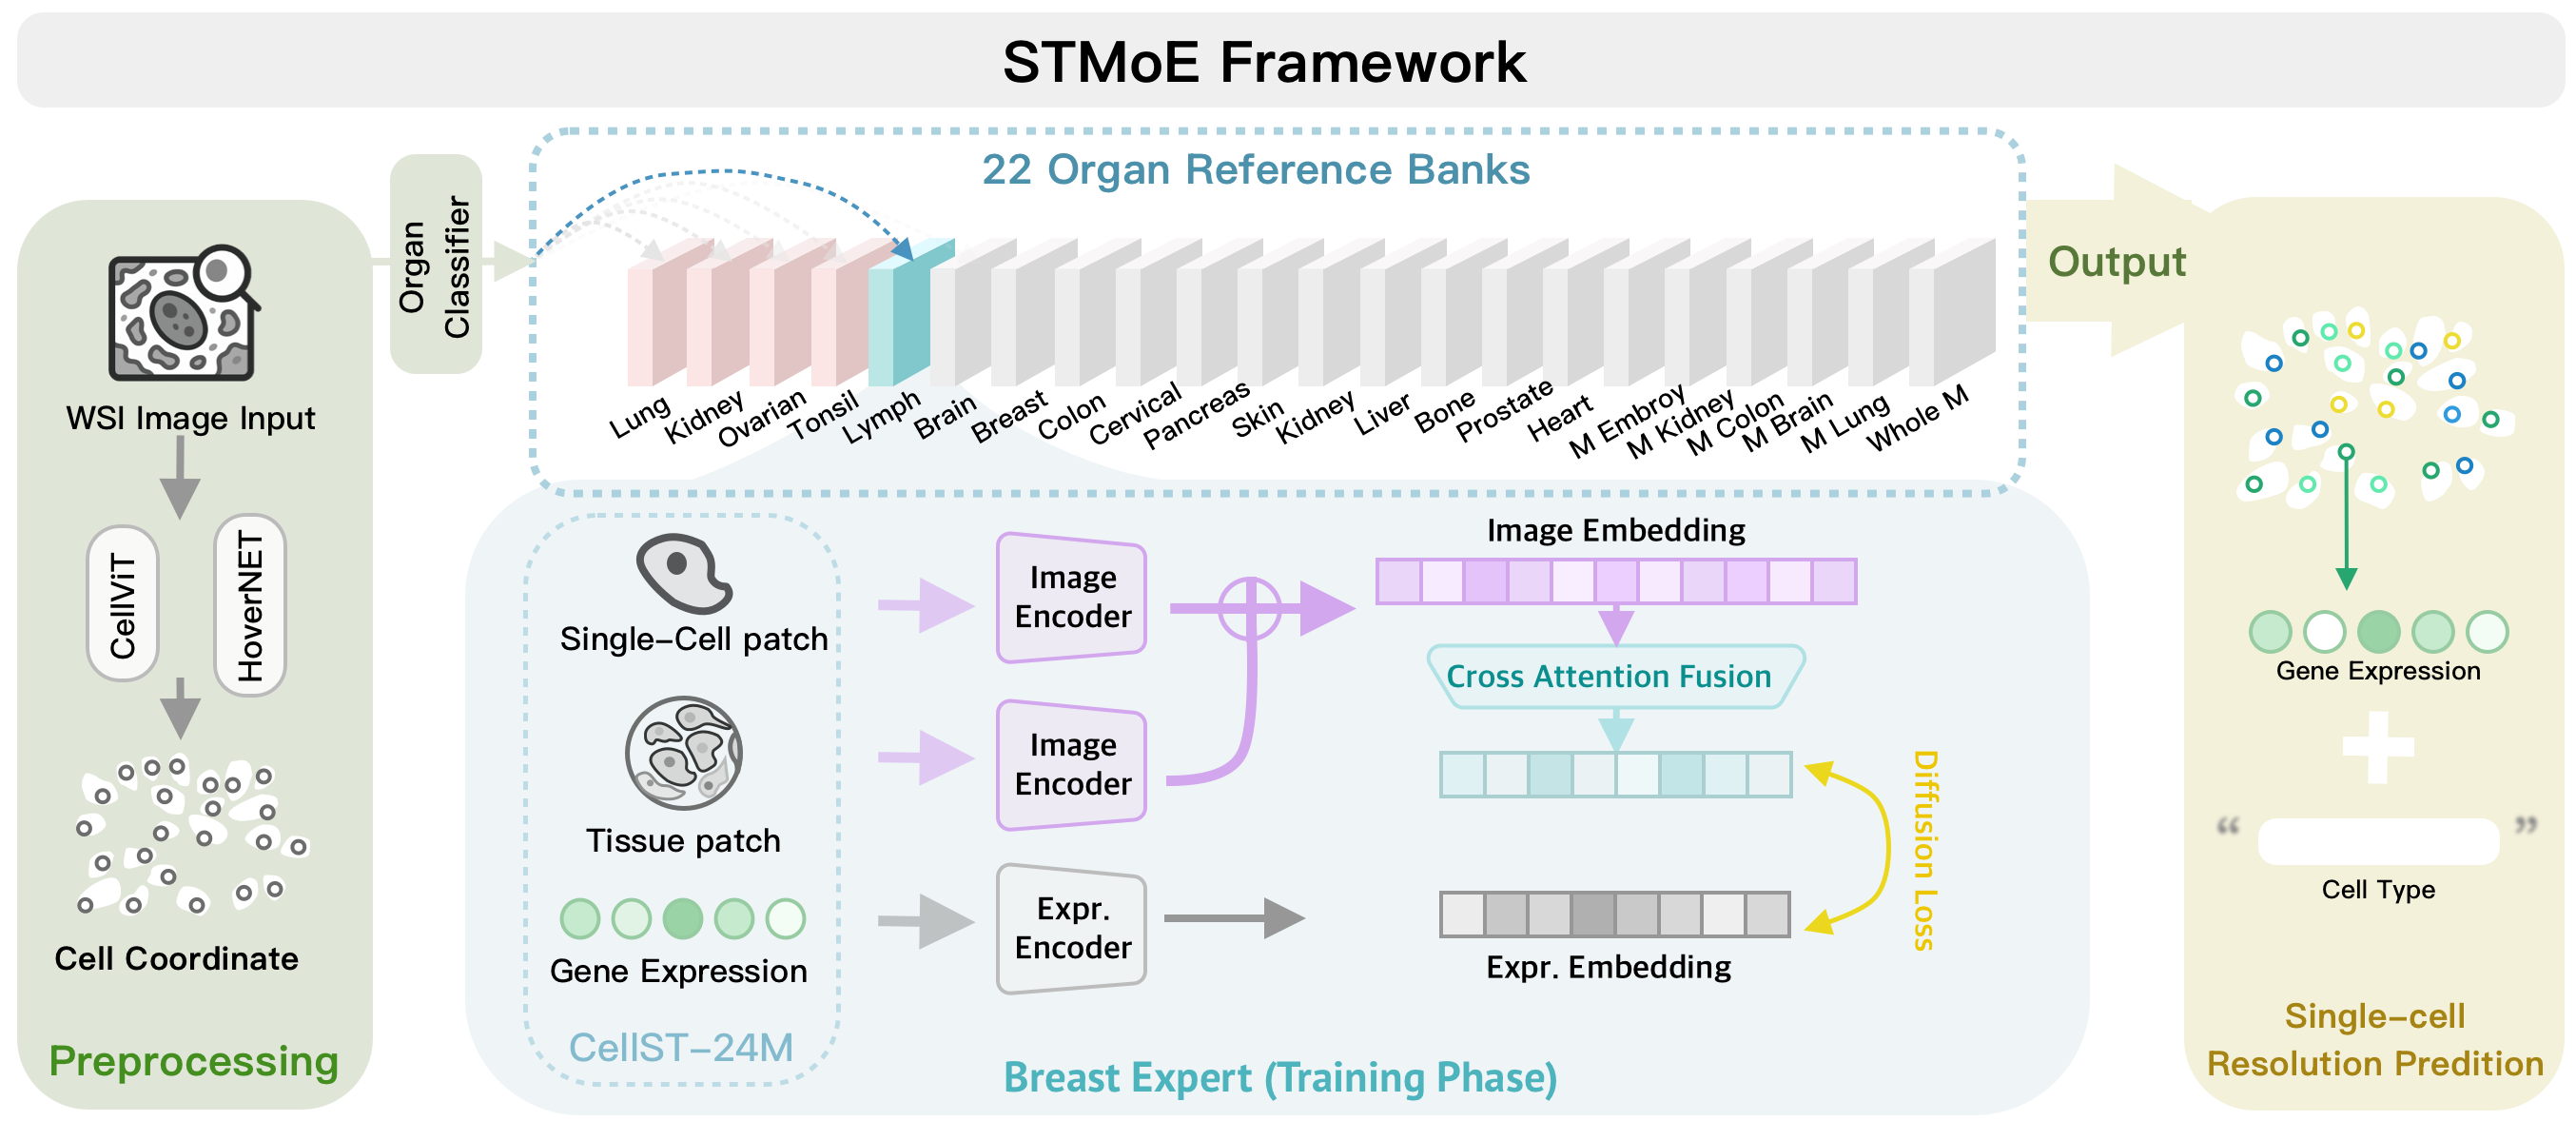
\includegraphics[width=0.98\textwidth]{model.png}
\caption{\method{} framework. During training, \dataset{} provides aligned cell records with local/context H\&E crops and measured expression profiles. A frozen UNI2-h encoder and an expression branch are aligned with a soft contrastive objective. During WSI-only deployment, CellViT++ detects cells, an organ classifier estimates routing weights, and full-gene expression is predicted by organ-routed retrieval from 22 training-only reference banks. Lung, kidney, ovary, tonsil, and breast have the largest banks and most stable evaluated predictions.}
\Description{Overview of STMoE. The training path uses CellST-24M aligned cell records with local and context histology crops and measured expression profiles. The inference path starts from a whole-slide image, detects cells with CellViT++, estimates organ routing weights, extracts image crops, and predicts full-gene expression through organ-routed retrieval.}
\label{fig:stmoe_architecture}
\end{figure*}

Here, we introduce \method{}, an organ-routed framework for WSI-only single-cell omics inference from histology (Fig.~\ref{fig:stmoe_architecture}). \method{} addresses the aligned-resource gap by building on \dataset{}, a large curated histology--transcriptomics resource with fixed leakage-controlled splits and training-only reference banks. It addresses the multi-organ deployment gap by combining WSI-derived cell detection with organ routing, allowing slides from different organs to share a common prediction interface while using organ-specific reference banks. It addresses the full-gene prediction gap by aligning image and expression embeddings with soft contrastive learning and predicting full-gene profiles through similarity-weighted retrieval from measured reference cells, avoiding a restricted marker-panel output or a parametric full-gene decoder.

To summarize, we make four contributions to single-cell histology-to-expression prediction:
\begin{itemize}[leftmargin=*]
    \item \textbf{Large dataset curation.} We curate \dataset{}, a 23.94M-cell histology--transcriptomics resource spanning 66 studies, 25 organ categories, Visium HD, and Xenium, with aligned cell records designed for leakage-controlled single-cell benchmarking.
    \item \textbf{Multi-organ full-gene prediction framework.} We introduce \method{}, a WSI-only organ-routed prediction framework that detects cells from H\&E slides, encodes cell-centered and tissue-context crops with UNI2-h, and predicts full-gene expression through organ-specific retrieval from training-only reference banks.
    \item \textbf{State-of-the-art strict cell-level performance.} On matched human lung benchmarks, \method{} outperforms representative baselines including cell-adapted BLEEP, sCellST and GHIST under in-domain and cross-patient evaluation.
    \item \textbf{Generalization and downstream validation.} Across 22 organs, \method{} supports direct multi-organ prediction, retains approximately 60\% predictive capability under cross-organ transfer, and recovers marker-derived coarse cell-type structure with 0.5935 accuracy and 0.5922 balanced accuracy.
\end{itemize}


\begin{table}[t]
\centering
\small
\setlength{\tabcolsep}{2.5pt}
\renewcommand{\arraystretch}{1.18}
\caption{Capability comparison with representative single-cell histology-to-expression methods. A red check mark denotes native support. A black cross denotes no native support. ``Direct multi-organ'' denotes native support for slides from multiple organs under one deployed interface. ``Full-gene'' denotes prediction over the full benchmark gene space rather than a restricted marker, panel, or spot-derived target subset.}
\label{tab:model_capability}
\begin{tabular}{@{}
>{\raggedright\arraybackslash}m{0.40\columnwidth}
>{\centering\arraybackslash}m{0.18\columnwidth}
>{\centering\arraybackslash}m{0.18\columnwidth}
>{\centering\arraybackslash}m{0.18\columnwidth}
@{}}
\toprule
\centering Method &
\shortstack{WSI-only\\inference} &
\shortstack{Multi-organ} &
\shortstack{Full-gene\\output} \\
\midrule
DeepSpot2Cell~\cite{Nonchev2025.09.23.678121} & \nomark & \nomark & \nomark \\
sCellST~\cite{chadoutaud2026scellst} & \yesmark & \nomark & \nomark \\
GHIST~\cite{fu2025ghist} & Partial & \nomark & \nomark \\
BLEEP (cell-adapted)~\cite{xie2023bleep} & \yesmark & \nomark & \yesmark \\
\rowcolor{blue!8}
\textbf{\method{} (ours)} & \textbf{\yesmark} & \textbf{\yesmark} & \textbf{\yesmark} \\
\bottomrule
\end{tabular}
\end{table}







\section{Related Work}

\textbf{Histology-to-expression and molecular prediction.}
Digital pathology has increasingly been used to infer molecular phenotypes from routine H\&E images. Early studies showed that histology can predict mutations, molecular subtypes, and transcriptomic signatures from weak slide- or patch-level supervision~\cite{coudray2018mutation,kather2020pancancer,pronier2020he2rna}. Spatial transcriptomics further enabled direct learning between local morphology and spatially indexed expression. ST-Net predicted breast-cancer gene expression from histology patches~\cite{he2020stnet}, while SpaCell integrated morphology and spatial expression for disease-cell prediction~\cite{tan2020spacell}. Later methods improved spot-level or super-resolved prediction using transformer, graph, contrastive, and multimodal architectures, including Hist2ST, HisToGene, BLEEP, TCGN, iSTAR, and THItoGene~\cite{zeng2022hist2st,pang2021histogene,xie2023bleep,xiao2024tcgn,zhang2024istar,jia2024thitogene,li2024ihast}. Recent benchmarking further shows that histology-to-expression prediction remains sensitive to tissue context, evaluation protocol, and translational setting~\cite{wang2025benchmark}. These works motivate our task, but most operate at the spot, tile, or super-resolution level rather than directly on aligned single cells.

\textbf{Single-cell histology-to-expression prediction.}
Single-cell expression prediction is more challenging because the target vector is sparse, noisy, and only partly reflected in the visible morphology of the target cell. Recent methods have begun to address this setting, but they often rely on additional non-image information or indirect supervision. GHIST predicts spatially resolved single-cell expression by combining morphology with cell type, neighborhood composition, and expression-related objectives~\cite{fu2025ghist}. sCellST predicts single-cell expression from H\&E images through weak supervision from spot-level spatial transcriptomics and multiple-instance learning~\cite{chadoutaud2026scellst}. In contrast, \method{} uses aligned cell-level records during training and requires only histology image inputs at inference: a cell-centered crop and a larger tissue-context crop. This keeps prediction cell-centered and image-only at deployment, while still allowing local tissue context to support genes that are not visually determined by the target cell alone.

\textbf{Spatial transcriptomics platforms, atlases, and benchmarks.}
Our work is also related to spatial transcriptomics technologies and reference resources. Array-based, sequencing-based, and imaging-based platforms provide spatial expression at different resolutions and gene coverages~\cite{stahl2016spatial,rodriques2019slideseq,stickels2021slideseqv2,vickovic2019hdst,chen2015merfish,eng2019seqfish,wang2018starmap,chen2022stereoseq,janesick2023xenium}. Large paired histology--omics datasets such as HEST-1K and STimage-1K4M support systematic benchmarking~\cite{jaume2024hest,chen2024stimage}, while single-cell atlases and spatial integration methods provide biological references for annotation and interpretation~\cite{regev2017hca,cziscience2025cellxgene,sikkema2023hlca,biancalani2021tangram,kleshchevnikov2022cell2location}. These resources are complementary to our objective: rather than mapping reference cells into space, we predict expression directly from histology for aligned cells.

\textbf{Pathology foundation models and multimodal pretraining.}
Large pretrained pathology encoders have become important building blocks for downstream histology tasks. Representative models include CTransPath, HIPT, UNI, CONCH, GigaPath, Virchow, Virchow2, Phikon, and H-optimus-0~\cite{wang2022ctranspath,chen2022hipt,chen2024uni,lu2024conch,xu2024gigapath,vorontsov2023virchow,zimmermann2024virchow2,filiot2024phikon,saillard2024hoptimus}. Vision--language pathology models and general medical-image pretraining further improve transferable and robust representation learning~\cite{huang2023plip,ikezogwo2023quilt,azizi2023remedis}. Broader LLM research examines robust rationalization, intent auditing, and cost-aware routing~\cite{zhang2025text,zhang2026position,zhang2026reasoning}. However, pathology encoders are not directly optimized for expression prediction, so we treat encoder choice as a separate scaling axis in our experiments.







\section{Large Dataset Curation: \dataset{} Enables Leakage-Controlled Cell-Level Benchmarking}

A central requirement for single-cell histology-to-expression modeling is a resource in which each training example is anchored to an individual cell rather than to a mixed spot or slide region. Existing resources partially support this goal: single-cell atlases provide cell-level molecular profiles but lack paired histology, pathology image--text corpora provide large visual pretraining data but lack expression targets, and spot-level ST resources provide paired histology and expression but aggregate multiple cells per target. \dataset{} closes this resource gap by curating a large cell-aligned histology--transcriptomics benchmark derived from public Visium HD and Xenium studies. The current release contains 23.94M aligned cell records across 66 studies and 25 organ categories, with each record linking a cell-level molecular target to a cell-centered H\&E crop, a larger tissue-context crop, spatial coordinates, platform metadata, and sample-level biological context.

\begin{table}[t]
\centering
\small
\setlength{\tabcolsep}{3pt}
\renewcommand{\arraystretch}{1.12}
\caption{Benchmark-oriented comparison with representative resources. ``Split'' indicates whether the resource natively supports predefined study-level or benchmark-level partitioning.}
\label{tab:resource_comparison}
\begin{tabularx}{\columnwidth}{@{}>{\raggedright\arraybackslash}Xccc@{}}
\toprule
Dataset & Single Cell & Multi-Organ & Split \\
\midrule
\rowcolor{gray!15}
\multicolumn{4}{@{}l}{\emph{Single-cell-only atlases}} \\
CELLxGENE Census~\cite{cziscience2025cellxgene} 
& Yes & Yes & Yes \\

\rowcolor{gray!15}
\multicolumn{4}{@{}l}{\emph{Pathology image--text corpora}} \\
OpenPath~\cite{huang2023visual} 
& No & Partial & No \\
Quilt-1M~\cite{ikezogwo2023quilt} 
& No & Partial & No \\
PathGen-1.6M~\cite{sun2024pathgen} 
& No & Partial & No \\

\rowcolor{gray!15}
\multicolumn{4}{@{}l}{\emph{ST + histology resources}} \\
HEST-1K~\cite{jaume2024hest} 
& No & Yes & Yes \\
STimage-1K4M~\cite{chen2024stimage} 
& No & Yes & Partial \\

\rowcolor{blue!10}
\textbf{\dataset{} (ours)}
& \textbf{Yes} & \textbf{Yes} & \textbf{Yes} \\
\bottomrule
\end{tabularx}
\end{table}

Compared with these resources, \dataset{} is designed around aligned cells as the benchmark unit (Table~\ref{tab:resource_comparison}). This makes it suitable for strict single-cell histology-to-expression evaluation rather than only spot-level, tile-level, or image--text pretraining. The release is organized as both a full aligned-cell resource and a set of benchmark-ready derived packages, including platform-specific \texttt{.h5ad} files, fixed split indices, configuration files, and a lightweight reviewer subset for smoke testing and figure/table regeneration (Table~\ref{tab:main_release_manifest}).

\begin{table*}[t]
\centering
\footnotesize
\setlength{\tabcolsep}{3pt}
\renewcommand{\arraystretch}{1.12}
\caption{\textbf{\dataset{} release manifest and benchmark coverage.}
Reviewer and benchmark packages are derived artifacts and do not introduce additional biological samples.}
\label{tab:main_release_manifest}
\begin{tabularx}{\textwidth}{
>{\raggedright\arraybackslash}p{1.55cm}
>{\raggedright\arraybackslash}p{1.45cm}
>{\raggedright\arraybackslash}p{1.35cm}
>{\centering\arraybackslash}p{0.75cm}
>{\raggedleft\arraybackslash}p{0.90cm}
>{\raggedright\arraybackslash}p{1.45cm}
>{\raggedright\arraybackslash}X
>{\raggedright\arraybackslash}p{1.55cm}
}
\toprule
\textbf{Block} &
\textbf{Platform} &
\textbf{Species} &
\textbf{Studies} &
\textbf{Cells} &
\textbf{Cell unit} &
\textbf{Benchmark coverage} &
\textbf{Files} \\
\midrule

Full release &
Xenium + Visium HD &
human, mouse, other &
66 &
23.94M &
Aligned cell &
In-domain, cross-patient, cross-platform, and context-shift evaluation &
\texttt{manifest/} \\

\addlinespace[1pt]

Xenium &
Xenium &
human, mouse &
42 &
16.31M &
Segmented cell &
In-domain and cross-platform single-cell evaluation &
\makecell[l]{\texttt{xenium/}\\\texttt{*.h5ad}} \\

Visium HD &
Visium HD &
human, mouse, other &
24 &
7.63M &
Bin-to-cell aligned &
In-domain, cross-patient, and cross-platform evaluation &
\makecell[l]{\texttt{visium\_hd/}\\\texttt{*.h5ad}} \\

\midrule

\rowcolor{gray!8}
Reviewer subset &
Mixed &
derived &
sub. &
rec. &
Cell-aligned &
Smoke testing and lightweight figure/table regeneration &
\makecell[l]{\texttt{review\_}\\\texttt{subset/}} \\

\rowcolor{gray!8}
Benchmark package &
Mixed &
mixed &
-- &
fixed &
Split-indexed &
In-domain benchmark for all organs; cross-patient and cross-platform protocols for eight organs &
\makecell[l]{\texttt{splits/}\\\texttt{configs/}} \\

\bottomrule
\end{tabularx}

\vspace{2pt}
{\footnotesize
\emph{Notes:}
The code and dataset release is available at
\protect\url{https://anonymous.4open.science/r/Orion-2053/}.
``Studies'' denotes standardized biological datasets included in the release.
``sub.'' and ``rec.'' indicate subset-level and record-level derived artifacts, respectively.
Cross-patient and cross-platform benchmarks are defined for eight multi-sample organs:
human breast, human ovary, human lung, human pancreas, human tonsil, mouse brain,
mouse embryo, and mouse kidney. All remaining organs are used for in-domain benchmarks.
\par}
\end{table*}

\dataset{} combines two complementary spatial-omics assay families. Xenium provides native cell-level measurements through platform-defined cell boundaries and transcript coordinates. Visium HD provides dense spatial expression bins and whole-slide histology; we convert these bins into cell-level targets by registering molecular coordinates to the histology frame, segmenting candidate cell footprints, aggregating overlapping bins to cells, and filtering records without stable expression support or valid image context. This curation step yields a common cell-aligned interface across assays: each retained cell has local morphology, neighborhood context, spatial coordinates, metadata, and an expression vector.

The construction pipeline follows the same record format across platforms. First, we audit each public source for tissue coverage, image availability, coordinate consistency, and usable molecular targets. Second, we define the cell unit: Xenium uses platform cell masks, whereas Visium HD uses a bin-to-cell conversion pipeline. Third, we extract two image views centered at each retained cell: a local crop for cell morphology and a larger crop for tissue context. Fourth, we harmonize expression targets within each evaluation regime. Within Visium HD, we use processed full-transcriptome targets; cross-platform experiments use only shared genes after symbol harmonization. Finally, we construct fixed benchmark splits for in-domain, cross-patient, cross-platform, and context-shift evaluation.

This curation also defines the prediction interface used in the rest of the paper. During training and evaluation, each retained cell provides a local crop $I_i^c$, a context crop $I_i^t$, an organ label $o_i$, and a processed expression vector $g_i$. The model learns an image--expression embedding space from the training split and predicts expression through retrieval from training-only reference banks:
\begin{equation}
    f_\theta(I_i^c, I_i^t; \mathcal{B}^{(o_i)}_{\mathrm{train}})
    \rightarrow
    \hat{g}_i \in \mathbb{R}^{G}.
\end{equation}
At WSI deployment, the query input is the slide image itself. Cell coordinates are obtained by CellViT++, organ identity is estimated by an organ classifier, and the same local/context crop interface is generated automatically from histology. In-domain evaluation uses spatially separated train and test regions from the same sample, while cross-patient evaluation trains on one sample and tests on a different sample with the same target-gene definition. These regimes are defined from curated \dataset{} split files rather than sampled ad hoc, keeping model and baseline comparisons matched in cells, genes, preprocessing, and metrics.





\section{Method}

\subsection{Overview}

\method{} predicts single-cell gene expression from histology through a retrieval-based image-to-expression framework trained on \dataset{}. The training unit is an aligned cell record: each retained cell is paired with a cell-centered H\&E crop, a larger tissue-context crop, and a measured expression profile. The two image crops are encoded by a shared frozen UNI2-h pathology foundation model and projected into a compact visual embedding. A paired expression branch maps reduced expression profiles into the same embedding space, and the two branches are aligned with a symmetric soft contrastive objective.

All training, validation, and test examples are defined by leakage-controlled \dataset{} split files. The split is fixed before model training, hyperparameter selection, and reference-bank construction. Test cells and their expression profiles are never used as retrieval references. In-domain, cross-patient, cross-study, and cross-platform regimes are therefore evaluated from predefined non-overlapping split files rather than from ad hoc sampling.

Unlike a parametric full-gene decoder, \method{} predicts expression through organ-routed retrieval. After contrastive alignment, a test cell is represented by its image embedding and retrieves similar expression-measured reference cells from the training split. The final full-gene expression vector is estimated as a similarity-weighted average of the retrieved reference profiles. Organ-specific reference banks allow the retrieval space to specialize across tissue contexts while preserving the same WSI-to-expression interface.

\subsection{Cell-Aligned Training Records and Reference Banks}

For each retained training cell $i$, \dataset{} provides a local crop $I_i^c$, a tissue-context crop $I_i^t$, a reduced expression representation $x_i$, a full-gene expression target $g_i$, an organ label $o_i$, and split metadata:
\begin{equation}
    r_i = (I_i^c, I_i^t, x_i, g_i, o_i).
\end{equation}
The local crop captures the target cell and immediate morphology, whereas the tissue-context crop captures nearby tissue organization and microenvironmental cues.

For each organ $o$, we define non-overlapping training, validation, and test sets:
\begin{equation}
    \mathcal{T}^{(o)}_{\mathrm{train}},
    \mathcal{T}^{(o)}_{\mathrm{val}},
    \mathcal{T}^{(o)}_{\mathrm{test}}.
\end{equation}
The retrieval reference bank is constructed only from $\mathcal{T}^{(o)}_{\mathrm{train}}$. Validation cells are used only for model selection, and test cells are excluded from both training and retrieval. This constraint is important for retrieval-based prediction because any leakage of test expression profiles into the reference bank would directly inflate performance.

\subsection{Multi-Scale Image and Expression Embedding}

For each cell $i$, we extract a local crop $I_i^c$ and a tissue-context crop $I_i^t$ centered at the same coordinate. In our implementation, the two crops are $64\times64$ and $256\times256$ pixels, respectively, and are resized to the UNI2-h input resolution. Both crops are encoded by the same frozen visual backbone:
\begin{equation}
    z_i^c = E_{\mathrm{UNI2\text{-}h}}(I_i^c), \qquad
    z_i^t = E_{\mathrm{UNI2\text{-}h}}(I_i^t).
\end{equation}
Using a shared frozen encoder keeps both image scales in the same representation space and limits trainable parameters to lightweight projection heads.

The two scale-specific embeddings are concatenated and passed through a residual projection head:
\begin{align}
    u_i &= [z_i^c; z_i^t], \\
    p_i &= W_p u_i, \\
    h_i^v &= \mathrm{LayerNorm}\left(
        p_i + \mathrm{Dropout}\left(W_o\,\mathrm{GELU}(p_i)\right)
    \right).
\end{align}
This produces a 256-dimensional visual embedding $h_i^v$.

During training, each cell also has a reduced expression representation $x_i$ derived from its measured expression profile. We map this vector into the same 256-dimensional embedding space using an expression projection head:
\begin{equation}
    h_i^g = P_g(x_i).
\end{equation}
The expression branch defines the molecular embedding space used for contrastive alignment and reference-cell retrieval. It is used only for cells with measured expression in the training/reference set; test-query cells are represented by image embeddings only.

\subsection{Soft Contrastive Alignment Objective}

We train the image and expression projection heads with a symmetric soft CLIP-style objective. For a minibatch of $n$ paired cells, image-expression logits are computed by dot-product similarity:
\begin{equation}
    \ell_{ij} = \frac{(h_i^g)^\top h_j^v}{\tau},
\end{equation}
where $\tau$ is the temperature.

Instead of using only one-hot paired labels, we construct soft targets from the average of image-image and expression-expression similarities:
\begin{equation}
    q_{ij}
    =
    \operatorname{softmax}_{j}
    \left(
    \frac{(h_i^v)^\top h_j^v + (h_i^g)^\top h_j^g}{2\tau}
    \right).
\end{equation}
The final loss is the average of expression-to-image and image-to-expression cross entropy:
\begin{equation}
    \mathcal{L}_{\mathrm{soft}}
    =
    \frac{1}{2}
    \left[
    \mathrm{CE}(\ell, q)
    +
    \mathrm{CE}(\ell^\top, q^\top)
    \right].
\end{equation}
This objective aligns matched image and expression embeddings while preserving neighborhood structure among biologically similar cells. Full-gene prediction is not learned through a parametric decoder; instead, the aligned embedding space is used for retrieval-based expression estimation.

\subsection{Organ-Routed Full-Gene Prediction}

After training, \method{} predicts full-gene expression by retrieving expression-measured reference cells from organ-specific training banks. For each organ $o$, we build an organ-specific reference bank:
\begin{equation}
    \mathcal{B}^{(o)}
    =
    \{(h_j^g, g_j): j \in \mathcal{T}^{(o)}_{\mathrm{train}}\}.
\end{equation}
Here, $h_j^g$ is the expression embedding of reference cell $j$, and $g_j$ is its full-gene expression profile. The reference bank is constructed only from the training split, so validation and test cells are excluded from retrieval.

For a query cell $i$ and organ $o$, we retrieve the $K_r$ nearest reference cells by image-to-expression similarity:
\begin{equation}
    \mathcal{N}^{(o)}_{K_r}(i)
    =
    \operatorname{TopK}_{j \in \mathcal{T}^{(o)}_{\mathrm{train}}}
    \left((h_i^v)^\top h_j^g\right).
\end{equation}
The retrieval weights are computed by a softmax over the selected references:
\begin{equation}
    w^{(o)}_{ij}
    =
    \frac{
    \exp((h_i^v)^\top h_j^g)
    }{
    \sum_{l \in \mathcal{N}^{(o)}_{K_r}(i)}
    \exp((h_i^v)^\top h_l^g)
    }.
\end{equation}
The organ-specific retrieval prediction is:
\begin{equation}
    \hat{g}^{(o)}_i
    =
    \sum_{j \in \mathcal{N}^{(o)}_{K_r}(i)}
    w^{(o)}_{ij} g_j.
\end{equation}

When the organ is known from the benchmark split, we use the corresponding organ-specific reference bank. For WSI deployment, an organ classifier provides organ-routing weights $a_o(S)$, and the final prediction is:
\begin{equation}
    \hat{g}_i
    =
    \sum_{o\in\mathcal{O}}
    a_o(S)\,\hat{g}^{(o)}_i.
\end{equation}
This organ-routed retrieval formulation provides organ-specific specialization without introducing a parametric full-gene decoder.




\subsection{WSI-Only Deployment Inference}
\label{sec:wsi_inference}

At deployment time, the input is a whole-slide H\&E image $S$. We first run two preprocessing modules. A cell-detection module, implemented with CellViT++, estimates cell locations:
\begin{equation}
    \{(x_i,y_i)\}_{i=1}^{N_S}
    =
    D_{\mathrm{cell}}(S).
\end{equation}
For each detected cell, we crop $I_i^c$ and $I_i^t$ centered at $(x_i,y_i)$ and encode them with the frozen UNI2-h image branch.

In parallel, an organ classifier estimates the organ identity or organ probability vector:
\begin{equation}
    a(S) = C_{\eta}(S), \qquad a(S)\in\Delta^{|\mathcal{O}|}.
\end{equation}


The organ prediction selects or weights organ-specific reference banks for retrieval. The query WSI does not require molecular measurements, external cell-type annotations, or manually provided neighborhood labels. Thus, deployment inference is WSI-only: cell locations, image crops, organ routing, and single-cell expression predictions are all produced from the input histology slide.










\begin{figure*}[t]
\centering
\includegraphics[width=0.98\textwidth]{main_exp.png}
\caption{Qualitative single-cell image-to-gene prediction on the matched lung benchmark. Top: in-domain A$\rightarrow$A evaluation. Bottom: cross-patient A$\rightarrow$B evaluation. Left panels compare tissue-level ground-truth and STMoE expression maps; right panels show representative H\&E neighborhoods with ground-truth and predicted expression patterns.}
\label{fig:main_exp}
\end{figure*}






\begin{table*}[t]
\centering
\small
\setlength{\tabcolsep}{3pt}
\renewcommand{\arraystretch}{1.15}
\caption{Multi-organ strict cell-level comparison against BLEEP~\cite{xie2023bleep}, GHIST~\cite{fu2025ghist}, and sCellST~\cite{chadoutaud2026scellst}. Results are reported on the five organs for which all baselines are available. BL, GH, SC, and ST denote BLEEP, GHIST, sCellST, and \method{}, respectively. Higher is better for all metrics, and bold values indicate the best method for each organ and metric.}
\label{tab:multi_organ_main}
\begin{tabular*}{\textwidth}{@{\extracolsep{\fill}}lrrrrrrrrrrrr@{}}
\toprule
& \multicolumn{4}{c}{Gene Pearson}
& \multicolumn{4}{c}{Gene Spearman}
& \multicolumn{4}{c}{Cell Pearson} \\
\cmidrule(lr){2-5}
\cmidrule(lr){6-9}
\cmidrule(lr){10-13}
Organ
& \makecell{BLEEP\\\cite{xie2023bleep}}
& \makecell{GHIST\\\cite{fu2025ghist}}
& \makecell{sCellST\\\cite{chadoutaud2026scellst}}
& \makecell{\method{}\\(ours)}
& \makecell{BLEEP\\\cite{xie2023bleep}}
& \makecell{GHIST\\\cite{fu2025ghist}}
& \makecell{sCellST\\\cite{chadoutaud2026scellst}}
& \makecell{\method{}\\(ours)}
& \makecell{BLEEP\\\cite{xie2023bleep}}
& \makecell{GHIST\\\cite{fu2025ghist}}
& \makecell{sCellST\\\cite{chadoutaud2026scellst}}
& \makecell{\method{}\\(ours)} \\
\midrule
Ovary
& 0.4239 & 0.4523 & 0.0800 & \textbf{0.6451} 
& 0.4396 & 0.4813 & 0.0640 & \textbf{0.6049}
& 0.8212 & 0.7382 & 0.6858 & \textbf{0.8379} \\

Lung
& 0.4241 & 0.4754 & 0.1255 & \textbf{0.5178}
& 0.4310 & 0.4814 & 0.1748 & \textbf{0.5077}
& 0.5622 & 0.5787 & 0.4704 & \textbf{0.6042} \\

Breast
& 0.0079 & 0.0487 & 0.0032 & \textbf{0.5118}
& 0.0051 & 0.0495 & 0.0070 & \textbf{0.5849}
& 0.1282 & 0.1832 & 0.1240 & \textbf{0.5465} \\

Kidney
& 0.3356 & 0.3040 & 0.0236 & \textbf{0.3643}
& \textbf{0.3468} & 0.2781 & 0.0264 & 0.3313
& \textbf{0.5369} & 0.5285 & 0.2601 & 0.5112 \\

Tonsil
& 0.1809 & 0.1591 & 0.0088 & \textbf{0.3817}
& 0.1794 & 0.1488 & 0.0084 & \textbf{0.3354}
& 0.7808 & 0.6107 & 0.7199 & \textbf{0.8193} \\
\bottomrule
\end{tabular*}
\end{table*}






\begin{table*}[t]
\centering
\footnotesize
\setlength{\tabcolsep}{1.2pt}
\renewcommand{\arraystretch}{1.10}
\caption{Representative gene-level results by organ. Sample identifiers are omitted. Each row reports gene name, expression mean, expression variance, and Pearson correlation.}
\label{tab:gene_examples}
\begin{tabular}{@{}lrrr@{\hspace{2pt}}lrrr@{\hspace{2pt}}lrrr@{\hspace{2pt}}lrrr@{\hspace{2pt}}lrrr@{}}
\toprule
\multicolumn{4}{c}{Ovary} &
\multicolumn{4}{c}{Lung} &
\multicolumn{4}{c}{Breast} &
\multicolumn{4}{c}{Kidney} &
\multicolumn{4}{c}{Tonsil} \\
\cmidrule(lr){1-4}
\cmidrule(lr){5-8}
\cmidrule(lr){9-12}
\cmidrule(lr){13-16}
\cmidrule(lr){17-20}
Gene & Mean & Var. & Pearson &
Gene & Mean & Var. & Pearson &
Gene & Mean & Var. & Pearson &
Gene & Mean & Var. & Pearson &
Gene & Mean & Var. & Pearson \\
\midrule
\rowcolor[gray]{0.92}
\multicolumn{20}{l}{\textbf{HVG (Highly Variable Gene)}} \\
MT-CO1 & 30.587 & 481.689 & 0.5211 &
IGKC & 4.528 & 293.750 & 0.4483 &
EVL & 0.134 & 0.254 & 0.2640 &
IGKC & 0.480 & 30.080 & 0.4551 &
CD74 & 18.546 & 332.186 & 0.3205 \\
MT-CO3 & 26.776 & 418.151 & 0.4869 &
IGHG1 & 1.858 & 65.348 & 0.4337 &
MYL9 & 0.121 & 0.226 & 0.3071 &
MT-CO3 & 2.024 & 7.732 & 0.4967 &
CLU & 4.141 & 61.560 & 0.4522 \\
MT-CYB & 18.797 & 226.742 & 0.4963 &
MT-CO3 & 4.939 & 57.392 & 0.6521 &
TRPS1 & 0.103 & 0.220 & 0.3155 &
IGHG1 & 0.122 & 2.229 & 0.4973 &
TMSB4X & 7.800 & 57.284 & 0.3285 \\
\addlinespace[2pt]
\rowcolor[gray]{0.92}
\multicolumn{20}{l}{\textbf{HEG (Highly Expressed Gene)}} \\
CD9 & 15.464 & 150.632 & 0.5012 &
MT-ATP6 & 3.043 & 20.250 & 0.6376 &
TAGLN & 0.125 & 0.202 & 0.2850 &
MT-CO1 & 1.041 & 2.037 & 0.3995 &
CCL19 & 2.975 & 31.486 & 0.3257 \\
MT-ATP6 & 15.245 & 145.242 & 0.4772 &
TMSB4X & 2.531 & 10.303 & 0.5497 &
SLC39A6 & 0.090 & 0.164 & 0.3313 &
MT-CYB & 0.984 & 2.166 & 0.4517 &
CD79A & 2.567 & 14.714 & 0.4282 \\
ERBB2 & 14.218 & 117.295 & 0.5408 &
CD74 & 2.268 & 9.902 & 0.4967 &
ACTA2 & 0.068 & 0.121 & 0.3687 &
MT-ATP6 & 0.884 & 1.721 & 0.3820 &
CD37 & 2.513 & 10.586 & 0.3325 \\
\bottomrule
\end{tabular}
\end{table*}


\section{Experiments}

We organize the experiments around the claims needed to support WSI-only, multi-organ, full-gene single-cell prediction. First, we define matched cells, leakage-controlled splits, and training-only reference banks to ensure that retrieval-based evaluation does not leak test expression profiles. Second, we test whether \method{} works beyond a single tissue by comparing it with representative baselines across organs. Third, we evaluate in-domain and cross-patient transfer on matched human lung benchmarks. Finally, we analyze encoder choice, retrieval size, reference-bank coverage, target space, image scale, and downstream cell-state consistency to explain where the performance gains come from.


\subsection{Data, Evaluation Protocol, and Training Details}

The main human lung benchmark uses two public 10x Genomics Visium HD CytAssist lung cancer datasets:
\begin{itemize}[leftmargin=*]
    \item \textbf{Sample A} is the Visium HD Spatial Gene Expression Libraries, Post-Xenium, Human Lung Cancer (FFPE) dataset, analyzed with Space Ranger 3.0.0~\cite{tenx2024visiumhd_lung_postxenium}.
    \item \textbf{Sample B} is the Visium HD Spatial Gene Expression Library, Human Lung Cancer (Fixed Frozen) dataset, analyzed with Space Ranger 3.1.1~\cite{tenx2024visiumhd_lung_fixedfrozen}.
\end{itemize}
We evaluate two matched regimes. In the in-domain A$\rightarrow$A regime, the left two-thirds of sample A are used for training and retrieval reference construction, while the spatially held-out right third is used for testing. In the cross-patient A$\rightarrow$B regime, the same sample-A training split is used, but evaluation is performed on sample B. Unless otherwise stated, all methods are evaluated on matched cells, matched target genes, and the same preprocessing pipeline.
\textbf{Cell-level target construction.}
Visium HD measures expression on a dense 8~$\mu$m bin grid rather than directly on segmented cells. We construct cell-level targets by registering molecular coordinates to the histology frame, segmenting candidate cell footprints, assigning overlapping bins to segmented cells, resolving boundary cases, and retaining cells with valid expression support and aligned image crops. For platforms with native cell-boundary support, such as Xenium, the platform mask and transcript coordinates define the cell unit directly. Each retained cell contains a cell identifier, spatial coordinate, local crop, context crop, sample metadata, and expression vector.

\textbf{Leakage-controlled splits.}
All training, validation, test, and retrieval reference sets are fixed before model fitting. In each benchmark regime, the retrieval reference bank is constructed only from the corresponding training split. Validation cells are used only for checkpoint selection and hyperparameter selection. Test cells and their expression profiles are excluded from both training and retrieval. This is essential for retrieval-based prediction because leakage of test expression profiles into the reference bank would directly inflate performance.

\textbf{Metrics.}
We report gene-wise Pearson and Spearman correlations, cell-wise Pearson and Spearman correlations, and sparse-expression F1 when applicable. Gene-wise metrics measure whether each gene's spatial variation is recovered across cells. Cell-wise metrics measure whether each cell's expression profile is recovered across genes. For sparse-expression recovery, we prefer rate-matched or row-wise top-$k$ F1 in baseline comparisons because default thresholded F1 can be distorted by different predicted nonzero rates.

\textbf{Baselines.}
We compare against a cell-adapted BLEEP baseline~\cite{xie2023bleep} under matched cell-level settings. In the expanded human lung benchmark, we additionally compare against DeepSpot2Cell~\cite{Nonchev2025.09.23.678121}, sCellST~\cite{chadoutaud2026scellst}, and GHIST~\cite{fu2025ghist}. Because these methods differ in their native supervision and deployment assumptions, we report all methods under the same strict cell-level evaluation protocol, and separately note when a method uses spot-derived supervision, additional non-image information, or a more favorable aggregated evaluation unit.

\textbf{Training details.}
For \method{}, we use MahmoodLab/UNI2-h as the frozen visual backbone with pretrained Hugging Face weights and an input resolution of $224\times224$. The local and tissue-context crops are $64\times64$ and $256\times256$ pixels, respectively, and are resized before encoding. Images are normalized with ImageNet mean and standard deviation. During training, we apply random horizontal flips, vertical flips, and rotations from $\{0^\circ,90^\circ,180^\circ,-90^\circ\}$.

The image and expression projection heads use a projection dimension of 256 and dropout of 0.1. We train the projection heads with AdamW using learning rate $1\times10^{-3}$, weight decay $1\times10^{-4}$, batch size 8, and temperature $\tau=1.0$, while keeping the UNI2-h backbone fixed. Models are trained for 10 epochs, and the checkpoint with the lowest validation loss is selected. Unless otherwise stated, retrieval uses $K_r=50$ nearest reference cells, selected from the retrieval-size sensitivity analysis in Table~\ref{tab:retrieval_sensitivity}.










\subsection{\method{} Outperforms Baselines Across Most Multi-Organ Cell-Level Metrics}

\method{} achieves the strongest overall multi-organ performance under strict cell-level evaluation, outperforming or matching representative baselines across most organs and metrics (Table~\ref{tab:multi_organ_main}). Across the five organs with complete baseline results, \method{} obtains the best score in 12 of 15 organ--metric comparisons. It is particularly strong for full-profile recovery, giving the best cell-wise Pearson in ovary, lung, breast, and tonsil. These results support the use of organ-routed retrieval as a shared multi-organ prediction interface rather than a single-organ model.

Representative gene-level results show that the recovered signal is not limited to a single marker family (Table~\ref{tab:gene_examples}). The retained examples include mitochondrial genes, immune-associated genes, epithelial markers, and tissue-structure-related genes, with several genes reaching strong Pearson correlations such as MT-CO3 in lung and ERBB2 in ovary. These examples support the main multi-organ result by showing that \method{} recovers heterogeneous gene-level signals rather than only one narrow marker type.










\begin{table}[t]
\centering
\small
\setlength{\tabcolsep}{3.5pt}
\renewcommand{\arraystretch}{1.14}
\caption{Human lung benchmark under strict cell-level evaluation. All methods are evaluated on matched cells and target genes within each regime. All reported metrics are correlations; higher is better.}
\label{tab:lung_benchmark}
\begin{tabular*}{\columnwidth}{@{\extracolsep{\fill}}lccc@{}}
\toprule
Method &
\makecell{Gene\\Pearson} &
\makecell{Gene\\Spearman} &
\makecell{Cell\\Pearson} \\
\midrule
\rowcolor[gray]{0.92}
\multicolumn{4}{@{}l}{\textbf{In-domain A$\rightarrow$A}} \\
BLEEP~\cite{xie2023bleep} & 0.4451 & 0.4066 & 0.5979 \\
sCellST~\cite{chadoutaud2026scellst} & 0.1281 & 0.1845 & 0.4832 \\
GHIST~\cite{fu2025ghist} & 0.4754 & 0.4814 & 0.5787 \\
\textbf{\method{} (ours)} & \textbf{0.5117} & \textbf{0.5069} & \textbf{0.6017} \\
\addlinespace[2pt]
\midrule
\rowcolor[gray]{0.92}
\multicolumn{4}{@{}l}{\textbf{Cross-patient A$\rightarrow$B}} \\
BLEEP~\cite{xie2023bleep} & 0.2248 & 0.2267 & 0.2592 \\
sCellST~\cite{chadoutaud2026scellst} & 0.0747 & 0.0681 & 0.1502 \\
GHIST~\cite{fu2025ghist} & 0.1959 & 0.1881 & 0.0844 \\
\textbf{\method{} (ours)} & \textbf{0.2986} & \textbf{0.2405} & \textbf{0.3451} \\
\bottomrule
\end{tabular*}
\end{table}









\begin{table*}[t]
\centering
\small
\setlength{\tabcolsep}{5pt}
\renewcommand{\arraystretch}{1.18}
\caption{Frozen pathology encoder comparison under a unified prediction protocol. H-optimus-0 is omitted. Bold values indicate the best result among the retained encoders for each metric. The highlighted row denotes the encoder selected for the final \method{} model.}
\label{tab:encoder_scaling}
\begin{tabular*}{\textwidth}{@{\extracolsep{\fill}}lcccccc@{}}
\toprule
& \multicolumn{3}{c}{Mouse} & \multicolumn{3}{c}{Human Lung} \\
\cmidrule(lr){2-4}
\cmidrule(lr){5-7}
Model &
\makecell{Avg.\\Pearson} &
Sensitivity &
Accuracy &
\makecell{Avg.\\Pearson} &
Sensitivity &
Accuracy \\
\midrule
ResNet50~\cite{he2016deep} &
0.4994 $\pm$ 0.0675 &
0.7927 $\pm$ 0.0140 &
0.6847 $\pm$ 0.0119 &
0.3629 $\pm$ 0.0860 &
0.6376 $\pm$ 0.0057 &
0.6222 $\pm$ 0.0004 \\

CTransPath~\cite{wang2022ctranspath} &
0.5058 $\pm$ 0.0611 &
0.7933 $\pm$ 0.0127 &
0.6865 $\pm$ 0.0097 &
0.3157 $\pm$ 0.1332 &
0.6287 $\pm$ 0.0146 &
0.6166 $\pm$ 0.0060 \\

Phikon~\cite{filiot2024phikon} &
0.4961 $\pm$ 0.0708 &
0.7918 $\pm$ 0.0149 &
0.6828 $\pm$ 0.0138 &
0.3690 $\pm$ 0.0799 &
0.6351 $\pm$ 0.0082 &
0.6187 $\pm$ 0.0039 \\

CONCH~\cite{lu2024conch} &
0.5145 $\pm$ 0.0524 &
0.7994 $\pm$ 0.0073 &
0.6905 $\pm$ 0.0061 &
0.3784 $\pm$ 0.0705 &
0.6361 $\pm$ 0.0072 &
0.6177 $\pm$ 0.0049 \\

UNI~\cite{chen2024uni} &
\textbf{0.5549} $\pm$ \textbf{0.0120} &
0.8051 $\pm$ 0.0016 &
0.6953 $\pm$ 0.0013 &
\textbf{0.4360} $\pm$ \textbf{0.0129} &
0.6416 $\pm$ 0.0017 &
0.6218 $\pm$ 0.0008 \\

\rowcolor{blue!8}
\textbf{UNI2-h}~\cite{chen2024uni} &
0.5545 $\pm$ 0.0124 &
\textbf{0.8067} $\pm$ \textbf{0.0000} &
\textbf{0.6966} $\pm$ \textbf{0.0000} &
0.4352 $\pm$ 0.0137 &
\textbf{0.6425} $\pm$ \textbf{0.0008} &
\textbf{0.6223} $\pm$ \textbf{0.0003} \\
\bottomrule
\end{tabular*}
\end{table*}



\begin{table}[t]
\centering
\small
\setlength{\tabcolsep}{2.5pt}
\renewcommand{\arraystretch}{1.12}
\caption{Reference-bank size, target-space, and image-scale ablations on the matched lung setting. Higher is better for all reported metrics. The highlighted row denotes the default configuration.}
\label{tab:ablation_components}
\begin{tabularx}{\columnwidth}{@{}>{\raggedright\arraybackslash}Xrrrrr@{}}
\toprule
Variant & Gene P & Gene S & Cell P & Cell S & F1 \\
\midrule
\rowcolor{gray!15}
\multicolumn{6}{@{}l}{\emph{Reference-bank size}} \\
20k references 
& 0.5318 & 0.5013 & 0.5901 & 0.5349 & 0.6291 \\
50k references 
& 0.5166 & 0.4911 & 0.5949 & 0.5332 & \textbf{0.6330} \\
\rowcolor{blue!8}
Full reference bank, $K_r=50$
& \textbf{0.5541} & 0.4867 & \textbf{0.6045} & 0.5430 & 0.5757 \\

\rowcolor{gray!15}
\multicolumn{6}{@{}l}{\emph{Target space}} \\
Train 50, eval 50 
& 0.5178 & \textbf{0.5077} & 0.6042 & \textbf{0.5452} & 0.6179 \\

\rowcolor{gray!15}
\multicolumn{6}{@{}l}{\emph{Image scale}} \\
No cell crop 
& 0.4482 & 0.3951 & 0.4876 & 0.4372 & 0.4628 \\
No context crop 
& 0.2163 & 0.1895 & 0.2352 & 0.2089 & 0.2215 \\
\bottomrule
\end{tabularx}
\end{table}




\begin{table}[t]
\centering
\small
\setlength{\tabcolsep}{3pt}
\renewcommand{\arraystretch}{1.12}
\caption{Retrieval-size sensitivity on the matched lung setting. $K_r=50$ is selected as the default because it improves continuous-expression correlation while avoiding the stronger over-smoothing observed at larger retrieval sizes.}
\label{tab:retrieval_sensitivity}
\begin{tabularx}{\columnwidth}{@{}>{\centering\arraybackslash}p{0.10\columnwidth}
>{\centering\arraybackslash}X
>{\centering\arraybackslash}X
>{\centering\arraybackslash}X
>{\centering\arraybackslash}X
>{\centering\arraybackslash}X@{}}
\toprule
$K_r$ & Gene P & Gene S & Cell P & F1 & Pred. rate \\
\midrule
1   & 0.4033 & 0.4154 & 0.5038 & 0.6280 & 0.2790 \\
5   & 0.4970 & 0.4820 & 0.5710 & \textbf{0.6530} & 0.4536 \\
10  & 0.5221 & \textbf{0.4915} & 0.5848 & 0.6329 & 0.5199 \\
20  & 0.5394 & 0.4909 & 0.5948 & 0.6080 & 0.5795 \\
\rowcolor{blue!8}
50  & 0.5541 & 0.4867 & 0.6045 & 0.5757 & 0.6477 \\
75  & 0.5588 & 0.4846 & 0.6079 & 0.5622 & 0.6751 \\
100 & \textbf{0.5623} & 0.4828 & \textbf{0.6101} & 0.5523 & 0.6950 \\
\bottomrule
\end{tabularx}
\end{table}











\subsection{\method{} Outperforms Cell-Level Baselines Under In-Domain and Cross-Patient Lung Transfer}

We next evaluate \method{} on matched human lung benchmarks against representative single-cell histology-to-expression baselines. The in-domain A$\rightarrow$A setting evaluates spatial generalization within the same sample, whereas the cross-patient A$\rightarrow$B setting evaluates transfer to a different patient sample with the same target-gene definition. This comparison is stricter than spot-level or tile-level prediction because every method is evaluated against cell-level expression targets.

Table~\ref{tab:lung_benchmark} summarizes the main human lung benchmark. In the current matched comparison with cell-adapted BLEEP, \method{} improves all three reported correlation metrics in the in-domain A$\rightarrow$A regime: gene-wise Pearson increases from 0.4451 to 0.5117, gene-wise Spearman from 0.4066 to 0.5069, and cell-wise Pearson from 0.5979 to 0.6017. These results indicate that \method{} better recovers continuous expression structure when training and testing are performed within the same sample under spatially separated splits.

The cross-patient A$\rightarrow$B setting is more challenging because it evaluates transfer to a different sample. In this regime, \method{} improves gene-wise Pearson from 0.2248 to 0.2986, gene-wise Spearman from 0.2267 to 0.2405, and cell-wise Pearson from 0.2592 to 0.3451. The gain is largest for cell-wise Pearson, suggesting that organ-routed retrieval preserves more profile-level expression correspondence under patient shift.

For the expanded benchmark, we evaluate DeepSpot2Cell, sCellST, GHIST, and cell-adapted BLEEP under the same in-domain and cross-patient protocol. We report the strict cell-level results as the primary comparison. When relevant, we also report spot-aggregated or native-granularity results as diagnostic analyses rather than as the main benchmark, because aggregation can smooth single-cell noise and produce a more favorable evaluation setting.



\subsection{Pathology Encoder Selection: UNI2-h Provides the Strongest Encoder}

Single-cell prediction depends strongly on the visual representation used by the downstream retrieval model. We therefore evaluate frozen histopathology encoders under a unified retrieval protocol on mouse brain and human lung benchmarks. Table~\ref{tab:encoder_scaling} reports average Pearson correlation, sensitivity, and accuracy across the compared encoders.

UNI and UNI2-h form the strongest retained encoder tier. UNI gives the highest average Pearson correlation on both mouse and human lung, while UNI2-h achieves the best sensitivity and accuracy on both benchmarks and remains within a very small margin of UNI in average Pearson. This trade-off makes UNI2-h a stable default encoder for the final \method{} model: it preserves near-best continuous-expression correlation while improving binary expression recovery and overall accuracy. We therefore use UNI2-h as the frozen pathology encoder in subsequent experiments.


\begin{figure*}[t]
\centering
\includegraphics[width=1.0\textwidth]{celltype.png}
\caption{Marker-derived downstream cell-state consistency on sample A. Coarse cell-state assignments are compared between ground-truth-derived and prediction-derived profiles using 111{,}772 aligned cells, 10 unsupervised clusters, and a restricted 50-gene target subset. The analysis focuses on three stable coarse classes: Club, AT2, and Immune.}
\label{fig:celltype_consistency}
\end{figure*}


\subsection{Ablation: Retrieval Neighborhood, Reference Coverage, and Image Scale Shape Prediction Quality}

Retrieval size controls a clear trade-off between continuous expression recovery and sparse nonzero-expression detection (Table~\ref{tab:retrieval_sensitivity}). Small retrieval neighborhoods preserve sparsity better: $K_r=5$ gives the highest F1 score, indicating the strongest nonzero-expression recovery, but its gene-wise and cell-wise Pearson correlations remain lower than larger retrieval neighborhoods. In contrast, increasing $K_r$ improves continuous correlation by averaging over more reference profiles. For example, $K_r=50$ improves gene-wise Pearson from 0.5221 to 0.5541 and cell-wise Pearson from 0.5848 to 0.6045 relative to $K_r=10$, while avoiding the stronger over-prediction observed at very large retrieval sizes. An additional $K_r=300$ run gives the highest Pearson values in the sweep, but its predicted nonzero rate rises to 0.7730 and F1 drops to 0.5147, indicating over-smoothing and excessive nonzero prediction. We therefore use $K_r=50$ as the default setting because the paper prioritizes continuous full-gene expression recovery while still maintaining a reasonable sparsity trade-off.

Reference-bank coverage further affects the quality of organ-routed retrieval (Table~\ref{tab:ablation_components}). After fixing the same retrieval setting, using the full reference bank gives the strongest continuous-expression recovery, reaching gene-wise Pearson of 0.5541 and cell-wise Pearson of 0.6045. Smaller reference banks remain competitive for sparse nonzero detection, with the 50k-reference setting achieving the highest F1 score of 0.6330, but they do not match the full bank on Pearson correlation. This supports using the full available training reference bank as the default when the goal is correlation-oriented full-gene prediction.

The target-space ablation shows a complementary trade-off. Direct 50-gene training with the full reference bank gives stronger gene-wise Pearson, whereas training on the full gene space and evaluating on 50 genes improves rank correlation, cell-wise Spearman, and F1. These results suggest that target-restricted training better optimizes continuous recovery on the evaluated gene subset, while full-gene training preserves broader expression structure and sparsity behavior.

Image-scale ablations confirm that both cell-centered morphology and tissue context are needed for robust prediction (Table~\ref{tab:ablation_components}). Removing the cell crop reduces gene-wise Pearson from 0.5541 to 0.4482 and cell-wise Pearson from 0.6045 to 0.4876, indicating that target-cell morphology contributes useful expression signal. Removing the context crop causes a much larger drop, reducing gene-wise Pearson to 0.2163 and cell-wise Pearson to 0.2352. This suggests that local tissue organization and neighborhood morphology provide essential cues for single-cell expression recovery. The full model therefore retains both image scales.







\subsection{\method{} shows strong performance on coarse cell-type prediction}

Although the primary task is gene-expression prediction, the predicted profiles should preserve enough biological structure to support downstream summaries. We run a marker-derived downstream analysis on the representative sample A using 111{,}772 aligned cells, 10 unsupervised clusters, and a restricted 50-gene target subset. Because this setup preserves stable signal for three coarse classes---Club, AT2, and Immune---we interpret it as a coarse cell-state recovery use case rather than a core benchmark task.

%\begin{figure}[t]
%\centering
%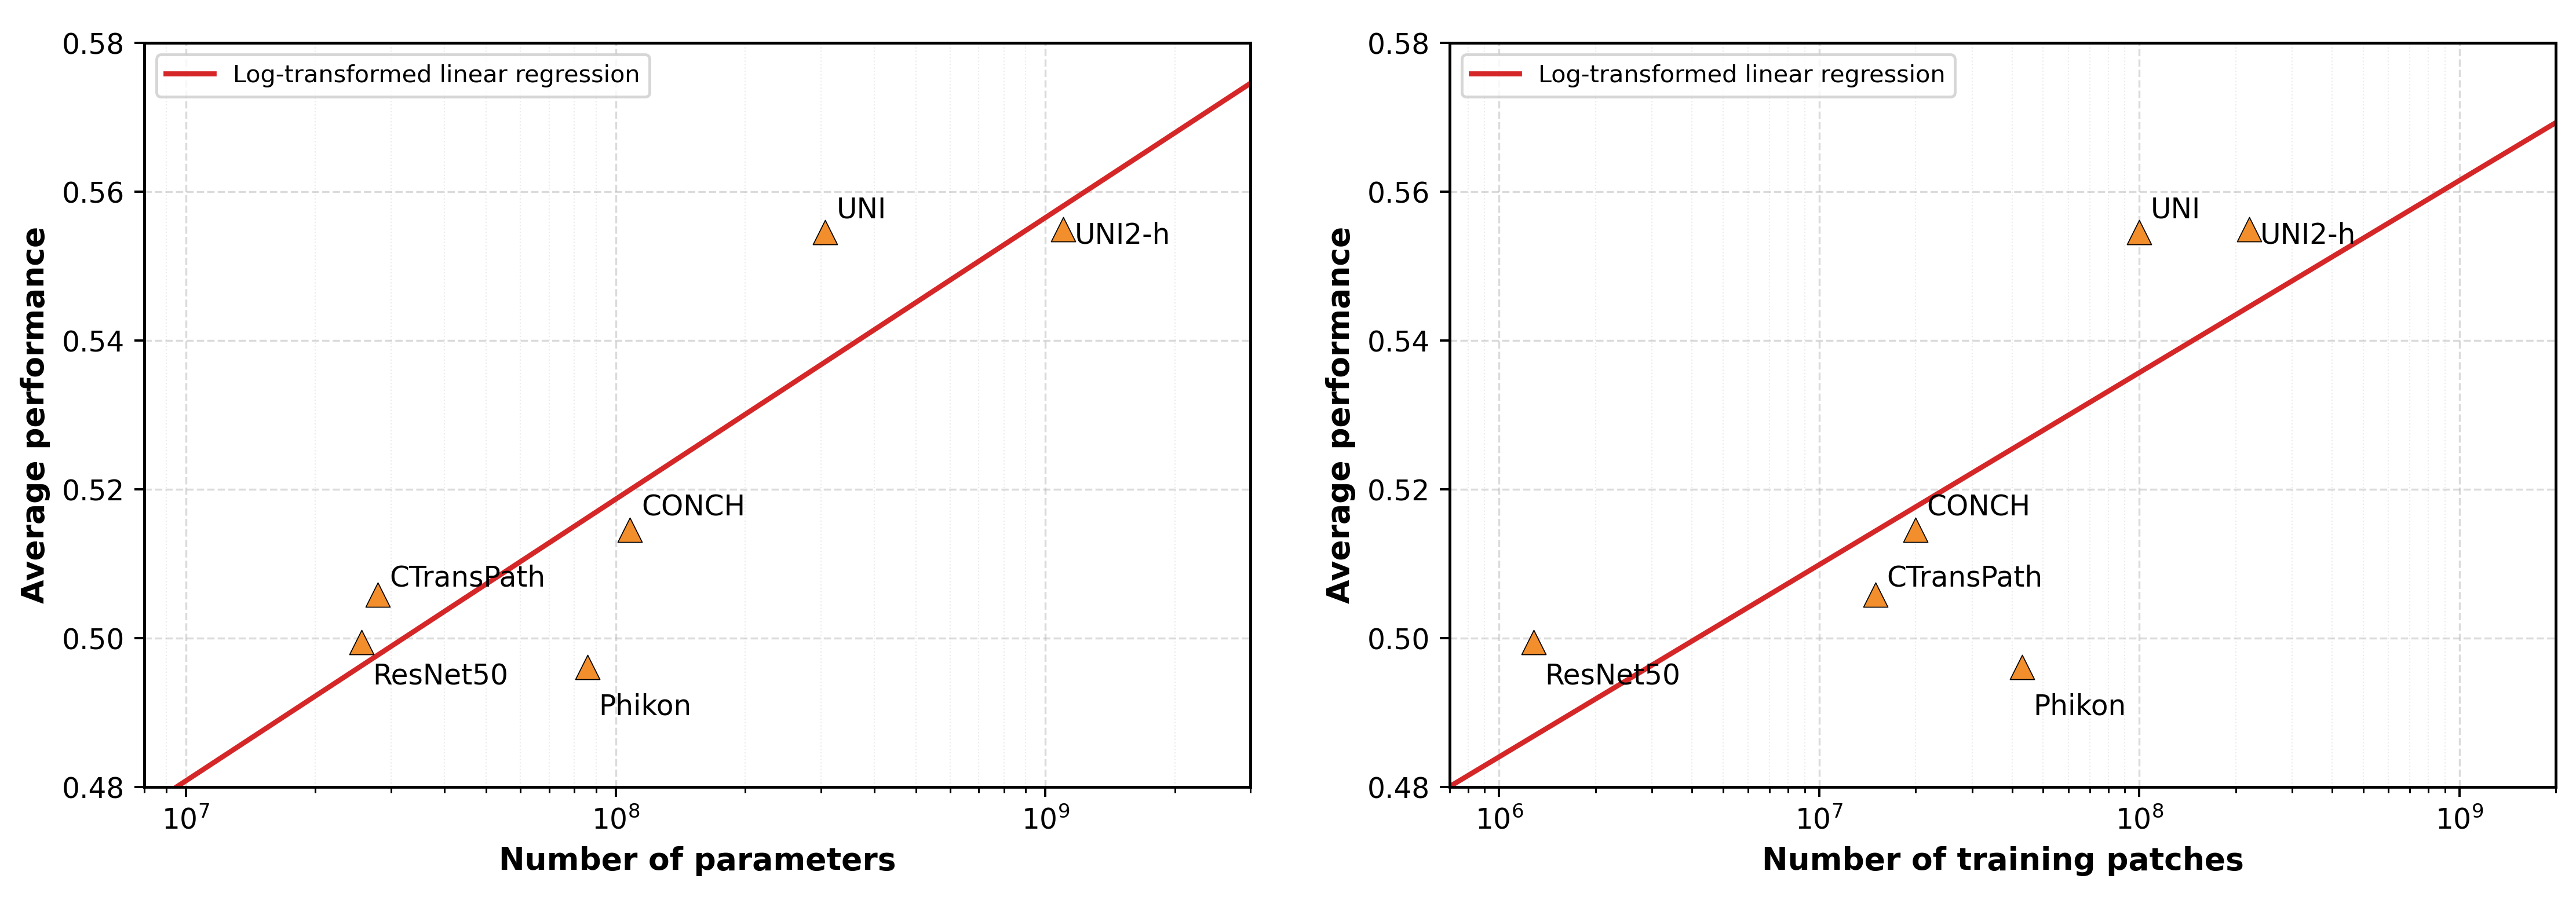
\includegraphics[width=0.5\textwidth]{encoder.png}
%\caption{Encoder-scaling trend for frozen pathology representations. Left: average Pearson performance versus the number of model parameters. Right: average Pearson performance versus the number of pretraining patches. Both x-axes use logarithmic scale, and the red line shows a log-transformed linear regression fit.}

%\label{fig:encoder_scaling_trend}
%\end{figure}





\begin{table}[t]
\centering
\small
\setlength{\tabcolsep}{5pt}
\renewcommand{\arraystretch}{1.12}
\caption{Global metrics for the representative sample-A downstream cell-state analysis. The analysis uses marker-derived coarse labels over a restricted 50-gene target subset.}
\label{tab:celltype_global}
\begin{tabularx}{\columnwidth}{@{}lX@{}}
\toprule
Metric & Value \\
\midrule
Cells & 111{,}772 \\
Clusters & 10 \\
Genes in downstream target & 50 \\
Cell-type accuracy & 0.5935 \\
Balanced accuracy & 0.5922 \\
Cluster--prediction ARI & 0.1362 \\
Cluster--prediction NMI & 0.2154 \\
Retained marker-derived classes & Club, AT2, Immune \\
\bottomrule
\end{tabularx}
\end{table}



As shown in Figure~\ref{fig:celltype_consistency}, the resulting coarse assignments reach 0.5935 accuracy and 0.5922 balanced accuracy. At the cluster level, all 10 clusters keep the same dominant coarse label between ground-truth-derived and prediction-derived assignments. The strongest agreement appears in a nearly pure Club cluster, cluster 3, with agreement 0.934. Several larger clusters also show robust agreement, including clusters 0, 2, 7, and 9, with agreement values of 0.639, 0.656, 0.550, and 0.670, respectively. The hardest cases are mixed Immune and AT2 clusters, especially clusters 1, 5, and 8, where agreement remains below 0.5 and the predicted composition becomes more diffuse. Table~\ref{tab:celltype_global} summarizes the corresponding global statistics. The moderate cell-level accuracy and balanced accuracy indicate partial recovery of coarse marker-derived states, whereas the lower ARI and NMI show that prediction-derived labels do not fully reproduce the unsupervised cluster structure. These results suggest that \method{} can preserve coarse tissue organization even when fine-grained single-cell expression recovery remains imperfect.

\section{Data and Code Availability}

The code, dataset manifest, benchmark splits, and reviewer subset are available at
\url{https://anonymous.4open.science/r/Orion-2053/}.


\section{Discussion}

\method{} addresses three practical gaps in single-cell histology-to-expression prediction: the lack of large aligned-cell resources, limited support for direct multi-organ deployment, and the difficulty of full-gene prediction from WSI-only inputs. CellST-24M provides the aligned-cell benchmark substrate, while \method{} converts a WSI into cell-level predictions through CellViT++ cell detection, organ routing, multi-scale UNI2-h image encoding, soft image--expression alignment, and retrieval from training-only reference banks. This design keeps inference WSI-only while allowing organ-specific specialization without a parametric full-gene decoder.

The results support this design across benchmark settings. In multi-organ evaluation, \method{} achieves the strongest overall performance across the five organs with complete baseline results, especially for cell-wise Pearson recovery. In matched human lung evaluation, \method{} outperforms cell-adapted BLEEP, sCellST, and GHIST under both in-domain and cross-patient regimes. The ablations show that retrieval size, reference-bank coverage, target space, and image scale all affect the balance between continuous-expression correlation and sparse-expression recovery. The downstream analysis further shows that predicted profiles preserve coarse cell-state structure, reaching 0.5935 accuracy and 0.5922 balanced accuracy.

Several limitations remain. Most importantly, cross-patient prediction is still less accurate than in-domain prediction. This gap likely reflects substantial patient-level context shift: differences in age, sex, comorbidities, treatment history, tissue processing, and disease state can change the global expression baseline even when the tissue morphology appears similar. Because current single-cell histology--transcriptomics resources remain limited in the number and diversity of matched patients, the reference banks do not yet fully cover these patient-specific expression shifts. Addressing this limitation will require larger multi-patient cohorts, better modeling of patient-level covariates, and calibration methods that separate morphology-driven signal from global patient-specific expression bias. This is a central direction for future work.

\section{Conclusion}

We presented \method{}, a WSI-only organ-routed prediction framework for single-cell gene-expression inference from histology, together with CellST-24M, a 23.94M-cell aligned histology--transcriptomics resource. \method{} combines cell-centered morphology, tissue context, soft image--expression alignment, and retrieval from training-only reference banks to predict full-gene profiles. Across multi-organ and matched human lung benchmarks, \method{} outperforms representative cell-level baselines and supports downstream coarse cell-state recovery. These results establish CellST-24M and \method{} as a benchmark and modeling framework for leakage-controlled, multi-organ, full-gene single-cell histology-to-expression prediction.

\begin{acks}
This work was supported by the National Institutes of Health under Award Numbers R01HG012572, R01NS128523, and R01DA063316.
\end{acks}



\section*{Generative AI Usage Disclosure}

Generative AI tools were used only for language polishing, structural editing, and LaTeX formatting assistance. All scientific claims, experimental design, data curation, model implementation, quantitative results, and conclusions were produced and verified by the authors. No patient-identifying information was provided to generative AI tools.

\bibliographystyle{ACM-Reference-Format}
\bibliography{stmoe_refs}

\end{document}
